\documentclass[a4paper, openany, 12pt]{article}

%% подключаем стандарт библиографии
\bibliographystyle{gost71u}

%% для "Abstract" в классе book
% \newenvironment{abstract}{}{}
% \usepackage{abstract}

%% подключаем преамбулу: в ней содержится подключение всех необходимых пакетов
%% Работа с русским языком
\usepackage{cmap}			 % поиск в PDF
\usepackage{mathtext} 		 % русские буквы в формулах
\usepackage[T2A]{fontenc}	 % кодировка
\usepackage[utf8]{inputenc}	 % кодировка исходного текста
\usepackage[russian]{babel}	 % локализация и переносы

%% Пакеты для работы с математикой
\usepackage{amsmath,amsfonts,amssymb,amsthm,mathtools}
\usepackage{icomma}

%% Нумерация формул (опционально)
%\mathtoolsset{showonlyrefs=true} % показывать номера только у тех формул, на которые есть \eqref{} в тексте.
%\usepackage{leqno}               % нумерация формул слева

%% Шрифты
\usepackage{euscript}	 % шрифт "Евклид"
\usepackage{mathrsfs}    % красивый мат. шрифт

%% Некоторые полезные макросы для дебага (в случае недоверия авторам шаблона)
\makeatletter
\newcommand\thefontsize{The current font size is: \f@size pt} % пример: \section{\thefontsize}
\makeatother

%% Настройка размеров шрифтов
\makeatletter
\renewcommand\Huge{\@setfontsize\Huge{14pt}{10}}
\renewcommand\huge{\@setfontsize\huge{14pt}{21}}
\renewcommand\Large{\@setfontsize\Large{14pt}{21pt}}
\renewcommand\large{\@setfontsize\large{12pt}{10}}
\makeatother

%% Поля (геометрия страницы)
\usepackage[left=3cm,right=1.5cm,top=2cm,bottom=2cm,bindingoffset=0cm]{geometry}

%% Русские списки
\usepackage{enumitem}
\makeatletter
\AddEnumerateCounter{\asbuk}{\russian@alph}{щ}
\makeatother

%% Работа с картинками
\usepackage[font=huge]{caption}
\captionsetup{justification=centering} % центрирование подписей к картинкам
\usepackage{graphicx}                  % вставки рисунков
\graphicspath{{images/}{images2/}}     % папки с картинками
\setlength\fboxsep{3pt}                % отступ рамки \fbox{} от рисунка
\setlength\fboxrule{1pt}               % толщина линий рамки \fbox{}
\usepackage{wrapfig}                   % обтекание рисунков и таблиц текстом

%% Работа с таблицами
\usepackage{array,tabularx,tabulary,booktabs} % дополнительная работа с таблицами
\usepackage{longtable}                        % длинные таблицы
\usepackage{multirow}                         % слияние строк в таблице

%% Красная строка
\setlength{\parindent}{2em}

%% Интервалы
\linespread{1}
\usepackage{multirow}

%% TikZ
\usepackage{tikz}
\usetikzlibrary{graphs,graphs.standard}

%% Верхний колонтитул
\usepackage{fancyhdr}
\pagestyle{fancy}

%% Перенос знаков в формулах (по Львовскому)
\newcommand*{\hm}[1]{#1\nobreak\discretionary{}{\hbox{$\mathsurround=0pt #1$}}{}}

%% Дополнительно
\usepackage{float}   % добавляет возможность работы с командой [H] которая улучшает расположение на странице
\usepackage{gensymb} % красивые градусы
\usepackage{caption} % пакет для подписей к рисункам, в частности, для работы caption*
\usepackage{listings} % пакет для листингов с кодом
\lstset{              % настройки для лисингов с кодом
basicstyle=\ttfamily,
columns=flexible,
breaklines=true,
captionpos=b
}
\usepackage[font=huge]{subcaption}

% Hyperref (для ссылок внутри  pdf)
\usepackage[unicode, pdftex]{hyperref}

% Отступ перед первым абзацем в каждом разделе
\usepackage{indentfirst}

\usepackage{sectsty}
\sectionfont{\fontsize{16}{21}\selectfont}
\subsectionfont{\fontsize{14}{21}\selectfont}
\subsubsectionfont{\fontsize{14}{21}\selectfont}
\paragraphfont{\fontsize{14}{21}\selectfont}


\begin{document}
    %% титульник
    \begin{center}
    %% *название института*
    \large\textbf{Министерство образования и науки Российской Федерации \\
    Московский физико-технический институт (государственный
    университет)} \\
    \vspace{1cm}

    %% *факультет/физтех-школа*
    Физтех-школа радиотехники и компьютерных технологий \\

    %% *название базовой кафедры и лаборатории*
    %% в случае ненадобности можно удалить
    Кафедра системного программирования ИСП РАН \\
    Лаборатория (laboratory name)\\

    \vspace{3em}

    Выпускная квалификационная работа бакалавра
\end{center}

\begin{center}
    \vspace{\fill}
    %% *название вашей работы*
    \LARGE{Разработка компилятора нейронных сетей на основе инфраструктуры MLIR для процессора с матричной архитектурой}

    \vspace{\fill}
\end{center}


\begin{flushright}
    \textbf{Автор:} \\
    Студент Б01-009 группы \\
    Вязовцев Андрей Викторович \\
    \vspace{2em}
    \textbf{Научный руководитель:} \\
    *научная степень* \\
    Денисов Денис Денисович \\
    \vspace{2em}
    \textbf{Научный консультант:} \\
    *научная степень* \\
    Сергеев Сергей Сергеевич \\
\end{flushright}

\vspace{7em}

\begin{center}
    %% *лого*
    \includegraphics[width=100 pt]{MIPT_logo.jpg}\\
    Москва \the\year{}
\end{center}

%% выключаем отображение номера для этой страницы (титульник)
\thispagestyle{empty}

\newpage
\setcounter{page}{2}
\fancyfoot[c]{\thepage}
%% *надпись над верхним колонтинулом*
%% в случае ненадобности можно удалить
\fancyhead[L]{Разработка компилятора нейронных сетей на основе инфраструктуры MLIR для процессора с матричной архитектурой}
\fancyhead[R]{}
    %% аннотоция
    \fontsize{14}{21}\selectfont
    \begin{abstract}

    \begin{center}
        \large{Разработка компилятора нейронных сетей на основе инфраструктуры MLIR для процессора с матричной архитектурой} \\
    \large\textit{Вязовцев Андрей Викторович} \\[1 cm]

    Краткое описание задачи и основных результатов, мотивирующее прочитать весь текст.

    \vfill

    \textbf{Abstract} \\[1 cm]

    FIXME: English abstract? 
    \end{center}

\end{abstract}
\newpage
    %% содержание
    \fontsize{14}{19}\selectfont
    \tableofcontents{}
    \newpage

    \fontsize{14}{21}\selectfont
    \section{Введение}
\label{sec:Intro} \index{Intro}

Нейронные сети в последниее время активно развиваются и находят применение
в большом количестве различных областей, в том числе очень популярными стали
средства для обработки естественной речи. Стоит отметить, что развитие
нейросетей происходит не только за счёт улучшения архитектура и точности
полученных ответов. Например, ведётся разработка способов ускорить исполнение
уже обученных моделей. Для этого разрабатываются процессоры с матричной
архитектурой, которые могут быть использованы в серверных или мобильных
решениях.

Для использования таких процессоров необходим широкий набор утилит, в том
числе и компиляторы. Как известно, основной задачей любого компилятора
является получение наиболее оптимального с точки зрения производительности
машинного кода при сохранении всех свойств исходной программы. Заметим, что в
таких компиляторах помимо традиционных техник оптимизации, таких как удаление
мёртвого кода, распостранения констант, сокращения общих подвыражений и других,
должны применяться другие техники, связанные с математическими свойствами
тензоров и спецификой целевой архитектуры.

В силу описанных выше причин идут активные исследования в области компиляторов
для нейронных сетей, в том числе и нашей лабораторией. В данной работе будет
исследованы особенности целевой архитектуры и представлены способы генерации
эффективого машинного кода.

\newpage

    \section{Постановка цели и задач}
\label{sec:Goals} \index{Goals}

Цель исследования: разработать компилятор нейронных сетей для процессоров
Ascend, основанных на архитектуре DaVinci \cite{ascend}, с использованием инфраструктуры
LLVM MLIR \cite{mlir-doc} и обеспечить генерацию эффективного машинного кода в нём.
Для достижения данной цели были поставлены следующие задачи:

\begin{enumerate}
    \item Исследовать архитектуру современных популярных нейронных сетей
          и типичные для них операции.
    \item Исследовать подходы к эффективному исполнению нейронных сетей,
          в том числе использование специальных процессоров (NPU),
          компиляторов с разными целевыми архитектурами (CPU, GPU, NPU),
          узнать их особенности и используемые в них оптимизации.
    \item Изучить инфраструктуру LLVM MLIR и предоставляемые ею возможности
          для написания собственного компилятора.
    \item Исследовать архитектуру DaVinci, принцип работы нейроматричного
          процессора и её язык ассемблера.
    \item Разработать набор операторов для целевой архитектуры DaVinci в
          инфраструктуре MLIR.
    \item Исследовать и предложить методы генерации оптимального машинного
          кода для некоторых типичных операций нейронных сетей.
    \item Реализовать наиболее эффективные способы генерации машинного кода,
          исследовать их производительность.
\end{enumerate}

\newpage

    \section{Обзор современных нейронных сетей}
\label{sec:Neuronets} \index{Neuronets}

\subsection{Общие соображения}

Искусcтвенная нейронная сеть --- математическая модель, а также её программное или
аппаратное воплощение, построенная по принципу организации биологических нейронных
сетей --- сетей нервных клеток живого организма. Этот принцип отражается в её
устройстве: нейронная сеть состоит из некольких слоёв, каждый из которых принимает
информацию с предыдущего, обрабатывает её каким-то образом, а  затем передаёт её
на следующий слой.

Благодаря новым исследованиям в этой области, нейронные сети нашли большое
количество применений в разных сферах жизни. В медицине они позволяют проводить
более точную диагностику заболеваний (например, онкологии), создавать портативные
устройтва для диагностики (например, для проведения ЭКГ). Они используются
для обработки больших данных в разных исследовательских областях, таких как
астрономия и геологоразведка. Также они упрощают жизнь в робототехнике и
автоматизации производства.

Рассмотрим наиболее популярные архитектуры нейронных сетей, их основные особенности.

\subsection{Обработка естественного языка}

Обработка естественного языка --- общее направление искусственного интеллекта и
математической лингвистики. Оно изучает проблемы компьютерного анализа и синтеза
текстов на естественных языках. Применительно к искусственному интеллекту анализ
означает понимание языка, а синтез --- генерацию грамотного текста. Одним из
подходов к решению данной задачи стала архитектура трансформер, представленная
компанией Google в 2017 году. Эта архитектура используется в переводчиках
(например, от компаний Яндекс и Google) и в чат-ботах (например, Chat GPT).
BERT, GPT-3, LLaMA --- модели, основывающиеся на архитектуре трансформер.

Многие из таких моделей можно скачать, после чего изучить их внутреннее
устройство. Нами была выбрана модель BERT. Не погружаясь в детали реализации
можно заметить, что подавляющее большиство операций в ней занимают
умножения матриц и поэлементные бинарные операции, такие как сложение и
умножение. Эти операции были выбраны для дальнейшего рассмотрения.

\subsection{Компьютерное зрение}

Компьютерное зрение --- теория и технология создания машин, которые могут
производить обнаружение, отслеживание и классификацию объектов. Распознавание
изображений может быть полезно в любой сфере, например, в сельском хозяйстве ---
для обнаружения болезни растений, в области безопасности --- для обнаружения
преступников и т.д.

Одно из наиболее популярных решений в этой области --- свёрточные нейронные
сети. Принцип их работы схож с работой зрительной коры головного мозга.
Основываются они на операции свёртки (конволюции). В функциональном анализе
она применяется к двум функциям и возвращает третью, соответствующую их
взаимной корреляции. Проще говоря, их можно интерпретировать как <<схожесть>>
двух функций.

В нейронных сетях свёртка применяется к изображениям, её схему можно увидеть
ниже. На часть изображения <<накладывается>> ядро, т.е. эта часть скалярно
умножается на ядро. Получившийся результат является каким-то признаком, он
записывается в результирующую матрицу --- матрицу выходных признаков
(output feature map). Стоит отметить, что общий случай свёркти несколько
сложнее, более подробно этот вопрос будет рассмотрен в соответствующей
главе.

\begin{figure}[h!]
    \centering
    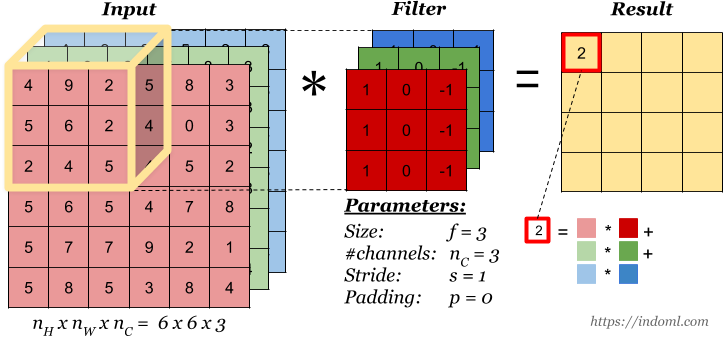
\includegraphics[scale=0.5]{Convolution.png}
    \caption{Операция свёркти для изображения с тремя цветами}
\end{figure}

Существует большое количество свёрточных нейронных сетей: LeNet-5, AlexNet,
VGG, GoogLeNet, ResNet, Inception. Нами была выбрана ResNet для дальнейшего
исследования. Она представлена несколькими вариантами, которые отличаются
количеством слоёв, а следовательно, точностью вычислений и размерами весов
модели. Модель с 18 слоями представлена на рисунке ниже. Как видно из
рисунка, в ней используются только операции свёркти. Но внутри них также
есть операции сложения и $Relu$, вычисляющейся по формуле \eqref{eq:Relu}.

\begin{equation}
    \label{eq:Relu}
    Relu(x) =
        \begin{cases*}
            x, ~ x \geqslant 0 \\
            0, ~ x < 0
        \end{cases*}
\end{equation}

\begin{figure}[h!]
    \centering
    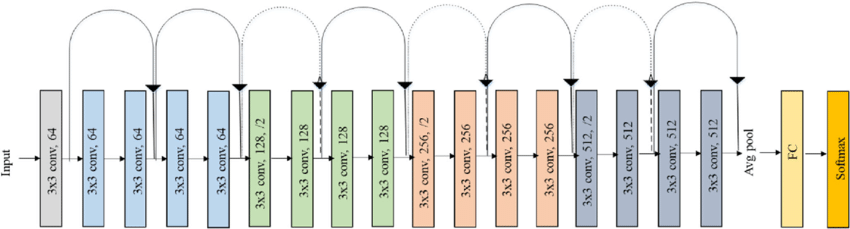
\includegraphics[scale=0.5]{ResNet18.png}
    \caption{Модель ResNet18}
\end{figure}

\newpage

    \section{Обзор существующих компиляторов нейронных сетей}
\label{sec:Compilers} \index{Compilers}

\subsection{Инфраструктуры и стандарты}

Для удобного проектирования, обучения и запуска нейронных сетей создаются
фреймворки (т.~е. библиотеки), поддерживающие большое количество операций
нейросетей и содержащие некоторые заранее натренированные модели и открытые
датасеты (наборы данных), использованные для их обучения. Наиболее популярными
из таких являются \textit{PyTorch} \cite{pytorch} и \textit{TensorFlow}
\cite{tensorflow}. Обучение и исполнение
моделей в этих фреймворках возможно как на CPU, так и на GPU.

Очевидно, что PyTorch и TensorFlow являются не единственными в своём роде.
По этой причине добавление возможностей исполнения на специализированном
процессоре в каждый фреймворк является нерациональным. Для унификации работы
с фреймворками, создаются стандарты, такие как \textit{ONNX} \cite{onnx},
\textit{TOSA} \cite{tosa} или \textit{StableHLO} \cite{stablehlo}.
Они создают единую точку входа для специализированных
компиляторов: сначала модель из любого фреймворка конвертируется в модель на
языке стандарта, и именно эту модель принимает на вход компилятор для создания
архитектурно-специфичного кода. Среди таких компиляторов можно выделить
\textit{XLA} \cite{xla}, \textit{MindSpore} \cite{mindspore},
\textit{ONNX runtime} \cite{onnx-runtime}. Но все они также
нацелены на исполнение на самых распростаннённых архитектурах (см. главу \ref{sec:Architecture}).
Их использование в качестве основы для создания
компилятора для архитектуры DaVinci означало бы написание полного цикла
компиляции из стандарта до ассемблерных инструкцию практически <<с нуля>> и
не давало бы никаких преимуществ. 

\subsection{Оптимизации и полиэдральная компиляция}
\label{subsec:poly}

Как было упомянуто ранее, одними из основных операций в нейронных сетях
являются умножения матриц и свёртки. Эти операции представляют из себя большое
количество простых и однотипных арифметических операций (сложения и умножения).
По этой причине их можно оптимизировать средствами векторизации и
переупорядочивания обхода циклов. Для этих целей была создана математическая
модель, основанная на алгебраическом представлении программ и их
преобразований, --- полиэдральная модель. В них цикл является полиэдром,
т.~е. многомерным многогранником в аффином пространстве. Аффинные преобразования
этого пространства соответствуют преобразованиям цикла, изменениям порядка
обхода элементов.

Рассмотрим некоторые проекты, использующие этот подход, а именно \textit{TVM}
\cite{tvm}, \textit{Halide} \cite{halide} и \textit{Polly} \cite{polly}.
Polly является частью проекта LLVM и
преобразует LLVM IR для генерации оптимального кода. Его использование привело
бы к необходимости добавления новых инструкций в LLVM IR и не давало бы
достаточных уровней абстракции. Инфраструктуры TVM и Halide позволяют
создавать новые операции, но требуют, чтобы для них был задан способ исполнения.
Такой подход является неудобным, т.~к. это означает, что после преобразований
код должен быть транслирован в ассемблерные инструкции по неким сложным
шаблонам. Более того, в Halide это исполнение задаётся исключительно скалярном
виде. К сожалению, единственный существующий компилятор для Ascend,
преобразующий ONNX модели, --- \textit{Automatic kernel generator (AKG)} \cite{akg},
являющийся частью MindSpore, пошёл по этому пути и использует Halide в качестве
инфраструктуры.

\subsection{Итог}

Существует большое количество различных компиляторов для нейронных сетей. Они
используют разлиные подходы для генерации кода, но во многом повторяют друг
друга. По этой причиной одно из крупнейших сообществ --- LLVM --- решило
создать переиспользуемую инфраструктуру MLIR, собирающую в себя лучшее из
различных подходов и техник, в т.~ч. и полиэдральной компиляции. На данный
момент проект активно развивается и является самой современной крупной
инфраструктурой.

\newpage

    \section{Обзор аппаратных решений}
\label{sec:Architecture} \index{Architecture}

\subsection{Оптимизации с помощью CPU, GPU и NPU}

Как было рассказано в главе про компиляторы, большинство современных библиотек
генерируют эффективный код для центральных процессоров (\textit{CPU},
\textit{central processing unit}) и графических процессоров (\textit{GPU},
\textit{graphics processing unit}). Рассмотрим технологии, которые они при
этом используют.

В случае CPU современным стандартом является технология \textit{AVX}
(\textit{advanced vector extentions}), которые позволяют использовать векторные
инструкции с длиной вектора 128, 256 или 512 бит. Большинство операций в
нейросетях являются векторными или матричными, по этой причине использование
их во время вычислений даёт прирост производительности в несколько раз по
сравнению со скалярным кодом. Но существуют и другие подходы. Добавляются
модули для матричных вычислений (\textit{AMX} у компании Intel, \textit{SME} в
архитектуре ARM), начиная с 2023 года в процессорах компаний Intel, AMD и
Qualomm начинают появляться нейропроцессоры (\textit{NPU},
\textit{neural processing unit}), специализированные для ускорения нейронных
сетей.

Другим классическим решением являются GPU, которые изначально предназначены
для параллельных однородных вычислений. Производители видеокарт создают
программные интерфейсы и их аппаратную поддержку для подобных целей. Таковыми
являются \textit{CUDA} у Nvidia и \textit{ROCm} у AMD. PyTorch и TensorFlow
поддерживают компиляцию с использованием этих технологий, время исполнения при
этом уменьшается в несколько десятков раз. Также отметим, что недавно в
графические ускорители добавили модуль матричных вычислений
(\textit{AMD matrix cores} и \textit{NVIDIA Tensor Cores}).

Распространение нейронных сетей во всех сферах жизни общества естественно
привело к созданию акселераторов, специализированных под них. Помимо модулей
в процессорах, упомянутых выше, существуют и другие решения. Таковыми являются
архитектура \textit{DaVinci} и процессоры \textit{Ascend} на её основе, которые
будут рассмотрены далее, \textit{LG NeuroMorphic Processor},
\textit{Google TPU}, а также российская разработка \textit{NeuroMatrix} от
НТЦ <<Модуль>>.

\subsection{Обзор архитектуры DaVinci}
\subsubsection{Общее описание}

Архитектура DaVinci --- нейропроцессор,разработанный компаней HiSilicon
(подразделение Huawei). В отличие от обычных CPU и GPU, которые необходимы
для вычислений общего назначения, и ASIC, предназначенной для конкретного
алгоритма, архитектура Da Vinci предназначена для исполнения уже обученных
нейронных сетей. Работа с NPU является обычной схемой гетерогенных вычислений,
в ней CPU является хостом (главным устройством, которое запрашивает вычисления),
а NPU --- девайсом (подчинённым устройством, производящим вычиления).
Взаимодействие между ними происходят по следующему алгоритму:

\begin{enumerate}
    \item Хост производит инициализацию, необходимую для общения с девайсом.
    \item Хост аллоцирует память (общую для него и девайса) и загружает данные в неё.
    \item Хост загружает объектный файл девайса и регистрирует функцию для исполнения.
    \item Хост передаёт указатели на аллоцированную память и даёт команду к исполнению.
    \item Девайс исполняет выбранную функцию.
    \item Хост копирует результат исполнения девайса к себе.
\end{enumerate}

Процессоры, основанные на архитектуре DaVinci и их основные характеристики
представлены в таблице ниже:

\begin{table}[h!]
    \centering
    \begin{tabular}{|c|c|c|c|c|}
        \hline
        Процессор & Производительность для float 16/int 8 & Мощность & Тех. процесс  \\ \hline
        Ascend 910 & 320/640~терафлопс & 310~Вт & 7~нм, N7+ \\ \hline
        Ascend 310 & 16/8~терафлопс & 8~Вт & 12~нм, FFC \\ \hline
    \end{tabular}
\end{table}

Теперь перейдём к внутреннему устройствую чипа Ascend. Схема архитектуры
представлена на рисунке. Рассмотрим её основные особенности.

\begin{figure}[h!]
    \centering
    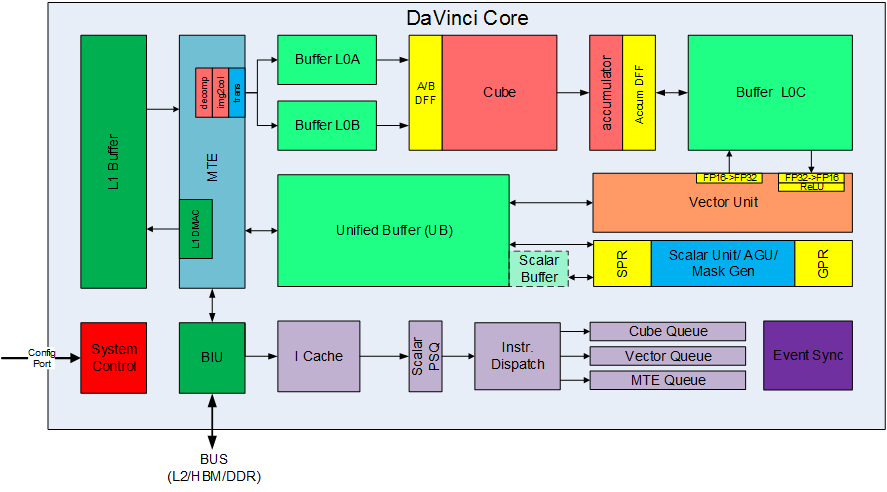
\includegraphics[scale=0.5]{DaVinci.png}
    \caption{Архитектура DaVinci}
\end{figure}

В ядре есть три вычислительных юнита: матричный, векторный и скалярный,
которые используются для соответствующих вычилений.  Исполнение на юнитах
происходит параллельно, для каждого юнита существует
отдельная, независимая очередь задач. Ещё три очереди предназначены для
копирования из разных буфферов друг в друга (о них речь пойдёт ниже).
Для синхронизации очередей используются команды \texttt{set\_flag},
\texttt{wait\_flag} и \texttt{pipe\_barrier}, которые по своей сути представляют
систему событий. Первая команда сигнализирует, что событие произошло, вторая
запускает ожидание события, а третья создаёт барьер, который означает
приостановку всех очередей до завершения какой-либо очереди. Правильное
использование механизмов синхронизации позволяет значительно увеличить
загрузку всех юнитов и, следовательно, снизить общее время исполнения.
В данной работе не будут рассматривать проблемы с расстановкой операций
синхронизации и будет считаться, что они всегда расставлены наиболее
оптимальным образом.

\subsubsection{Матричный юнит}

Матричный юнит на вход принимает матрицы с типом элементов \texttt{float 16}
или \texttt{int 8}, на выходе же элементы имеют тип \texttt{float 16},
\texttt{float 32} или \texttt{int 32}. Умножение работает в двух режимах:

\begin{enumerate}
    \item Обычное умножение: $C = A \times B$
    \item Режим накопления: $C = A \times B + C$, т.~е. результат текущего
          умножения прибавляется к предыдущему.
\end{enumerate}

Каждая из входных матриц должна быть разбита на блоки $16 \times 16$
(в случае \texttt{float 16}) или $16 \times 32$ (в случае \texttt{int 8}).
Расположение элементов внутри блоков и блоков относительно друг друга также
различно. Существуют две стратегии размещения: про строкам (формат \texttt{Z})
и по столбцам (формат \texttt{N}). Примем обозначение: размещение внутри блока
обозначается строчной буквой, а между блоками --- заглавной. При умножении
матрица $A$ должна быть заранее быть записана в формате \texttt{Zz},
матрица $B$ --- в формате \texttt{Zn}, а выходная матрица $C$ будет \texttt{Nz}.

Матричный юнит работает по принципу систолического массива.
Систолический массив --- однородная сеть тесно связанных блоков обработки данных.
Его схему для архитектуры DaVinci можно увидеть на картинке ниже.

Принцип умножения довольно прост: за первый такт происходят все умножения,
после чего за оставшиеся четыре такта произведения суммируются. Таким
образом, за пять тактов можно перемножить две матрицы \texttt{16x16}.
Матричный юнит, итерируясь по матрицам и перемножая их поблочно, быстро
получает результат перемножения.

\begin{figure}[h!]
    \centering
    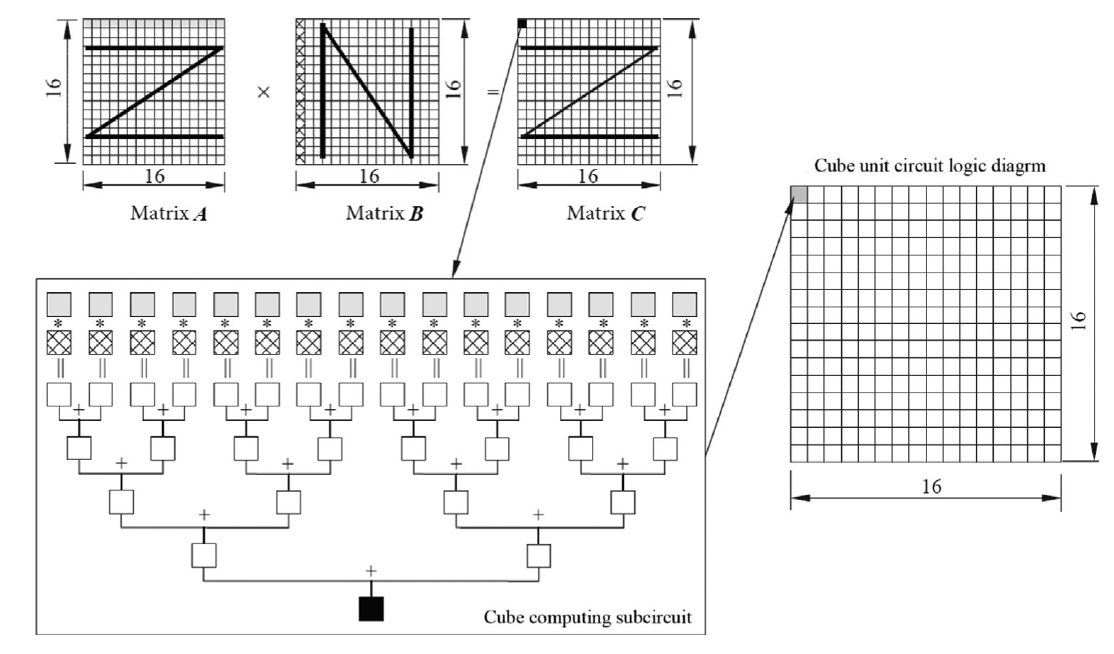
\includegraphics[scale=0.5]{Systolic.png}
    \caption{Схема вычисления в матричном юните}
\end{figure}

\subsubsection{Векторный юнит}

Теперь рассмотрим работу векторного юнита. Существуют два режима работы:
\textit{common} и \textit{VA}. В обоих случаях память делится на блоки
по 32 байта, а векторная операция представляется в виде цикла, на каждой
итерации которого обрабатывается 8 блоков. Таким образом, за одну итерацию
может быть обработано 128 элементов типа \texttt{float 16} или 64 элемента
32-разрядных типов (\texttt{float 32}, \texttt{int 32}). Стоит отметить, что
не обязательно обрабатывать такое количество элементов. Для выбора, с какими
именно элементами будет работать операция необходимо задать маску. Векторный
юнит обрабатывает только те элементы, на позиции которых в маске стоит бит 1.
На каждой следующей итерации блоки сдигаются на заранее заданный шаг,
после чего операция повторяется. Отличаются режимы способом описания этих блоков.
В случае \textit{VA} режима блоки задаются в виде восьми указателей, а в случае
\textit{common} --- указателем на первый блок и шагом между блоками. Для первого,
второго аргумента и результата шаг может быть различным. 
Юнит поддерживает большое количество операций: математических, логических,
приведения типов и т.~д. Есть и спецефичные операции: \textit{relu}, часто
используемый в нейронных сетях, операция транспонирования.

\subsubsection{Память}

Память ядра неоднородна. В ядре существует 5 буферов:
L1, L0A, L0B, L0C, UB. Также существует внешняя память (GM), через которую
происходит общение с хостом. Опишем общую схему потока данных между этими кэшами.
Данные из внешней памяти загружаются в L1 или UB. Данные в UB предназначены для
обработки векторным и скалярным юнитами. Данные из L1 загружаются в L0A и L0B,
которые соответствуют матрицам A и B матричного умножения. Результат после
перемножения (которое, как было упомянуто раньше, выполняется матричным юнитом),
попадает в буфер L0C, из которого происходит данные отправляются в UB. Выгрузка
результата вычислений во внешнюю память возможна только из UB. Отметим, что
описанные выше буферы имеют небольшой размер, что будет значительно влиять на
построение стратегий эффективного исполнения операций. Также буферы являются
\textit{гранулярными}, в L1 и UB загрузка и выгрузка происходит блоками по 32
байта, а в L0A, L0B и L0C --- по 512.

\subsubsection{Свёртка}

Реализация свёртки на нейроматрицных процессоров несколько сложнее, чем умножения.
На некоторых архитектурах (FIXME: ссылка) она поддержана нативно. К сожалению, наша
не является таковой. Но с помощью особого преобразования её можно свести к 
умножению матриц. Приведём некоторые общие соображения, которые позволят понять его.

Итак, пусть есть входное изображение (\textit{image}) размеров $H_i \times W_i$,
содержащее $C$ цветов. Будем называть его \textit{входной картой признаков}
(\textit{input feature map}). Ядро (\textit{kernel}) свёртки представляет из
себя небольшую матрицу размеров $H_k \times W_k$ (характерный размер --- $3-5$).
Ядро имеет такое же количество входных цветов $C$, но также имеет и $F$
выходных цветов. Таким образом, изображение имеет формат $H_i W_i C$,
а ядро --- $F H_k W_k C$. Выходная карта признаков, имеет структуру, схожую
со входной: $H_o W_o F$, где $H_o = H_i - H_k + 1$, $W_o = W_i - W_k + 1$
в простейшем случае. Если обозначить: $a$ --- входная карта, $k$ --- ядро,
$c$ --- выходная, то свёрка выражается следующей формулой:

\[
    c_{ijf} = \sum \limits_{h = 0}^{H_k} \sum \limits_{w = 0}^{W_k}
              \sum \limits_{c = 0}^{C} a_{i+h, j+w, c} \cdot k_{f h w c}
\]

Заметим, что операция чем-то схожа на скалярное умножение векторов
(если цвета считать вектором) или матричное умножение. Если первый тензор
преобразовать в матрицу $A$, где одной строке будет соответвовать одна
такая сумма (т.е. размеры матрицы станут $H_o W_o \times H_k W_k C$), а
ядро --- в матрицу $K$ размеров $H_k W_k C \times F$, то выходная
матрица $C = A \times K$. Этот процесс преобразования входной карты
признаков называется \textit{img2col} (\textit{image-to-column}),
оно содержится в архитектуре команд целевого процессора.

Таким образом, свёрка есть композиция \textit{img2col} и умножения матриц.
Отметим, что в реальности свёртка имеет такие параметры, как
\textit{stride}, \textit{dilation} и \textit{pad}. Они усложняют
приведённые формулы, но не меняют сути происходящего. Также в
качестве обобщения можно взять $N$ изображений, форматы входной и
выходной карт приобретают вид $N H_i W_i C$ и $N H_o W_o F$ соответственно.

\subsubsection{Изменение формата хранения данных}

Рассмотрим принцип работы инструкции \textit{scatter\_vnchwconv}. Она будет
использоваться в операциях, где необходимо изменить формат хранения данных
(например, транспонировать матрицу). За одну итерацию операция работает с
двумя матрицами $16 \times 16$ типа \texttt{float 16}. Каждая матрица задаётся
16-ю указателями на строки, строки не обязаны <<лежать подряд>>. Исходная
матрица транспонируется и записывается по соответствующим указателям выходной
матрицы. При переходе на следующую итерацию указатели сдвигаются на некоторый
шаг (общий для всех 16-ти указателей, но различный для входной и выходной
матриц).

\subsubsection{Возможные оптимизации}

Рассмотрим некоторые оптимизации, которые применимы на архитектуре DaVinci:

\begin{enumerate}
    \item Разбиение задачи на несколько потоков. В процессорах Ascend несколько
          ядер на архитектуре DaVinci, поэтому задачу можно разбивать на
          несколько параллельных (например, в случае умножения матриц ---
          воспользоваться блочным умножением).
    
    \item Двойная буферизация. Как было описано выше, ядро процессора имеет
          несколько вычислительных юнитов, работающих параллельно. Чем больше
          юнитов работают одновременно, тем быстрее завершится исполнение
          задачи. Сделаем одновременным работу модуля памяти и какого-нибудь
          вычислительного модуля. Для этого разделим буфер на две части. Пока
          в первом будет происходить загрузка или выгрузка, в другом
          производятся вычисления. 
\end{enumerate}

\newpage

    \section{Структура компилятора и его реализация}
\label{sec:Chapter7} \index{Chapter7}

\subsection{Инфраструктура LLVM MLIR}
\label{impl:mlir} % \index{Chapter5}

Как можно заметить из предыдущего параграфа, компиляторы из предыдущего параграфа
решали сходные задачи, но они отличались некоторыми деталями, из-за чего
приходилось создавать новый компилятор и пересоздавать большое количество
компонентов. В связи с этим сообщество разработчиков LLVM придумали и реализовали
переиспользуемую и расширяемую инфраструктуру MLIR.

Основная концепция MLIR --- диалекты. Диалект объединяет в себе типы, операции
и их преобразования на каком-либо уровне абстракции. В MLIR существует более 40
встроенных диалектов, имплентация собственных диалектов возможна с помощью
декларативного языка \textit{ODS} или на языке C++.

Рассмотрим некоторые диалекты, которые будут использованы в данной работе.

\begin{enumerate}
    \item HLO --- диалект, который позволяет представлять модели нейросетей,
          написанных на tensorflow, в представлении MLIR. Несмотря на то,
          что он не является стандартным и представлен в виде отдельного
          репозитория, пользуется популярностью благодаря широкой
          известности tensorflow.

    \item tensor --- диалект для представления тензоров и операций,
          позволяющих менять форму тензоров, изменять их размеры,
          <<вырезать>> и <<вставлять>> части из них. Стоит отметить, на
          данном уровне абстракции считается, что тензоры не имеют какого-то
          конкретного расположения в памяти. Этим они похожи на виртуальные
          регистры из теории компиляторов.

    \item memref --- диалект, который абстрагирует работу с многомерными
          массивами. Операции в этом диалекте схожи с операциями из диалекта
          tensor, но этих диалектов есть существенное отличие: memref является
          представлением реальных объектов.

    \item affine --- диалект, который предоставляет возможность работы с
          аффинными циклами и преобразованиями над ними, тем самым реализуя
          возможности для полиэдральной компиляции.

    \item scf (structured control flow) --- диалект, в котором представлен
          структурный поток исполнения (т.е. в виде системы вложенных блоков).

    \item cf (control flow) --- диалект, предсталяющий исполнение в виде графа
          потока управления.

    \item func --- диалект, реализующий концепцию функций, их вызова, передачи
          аргументов, возвращения значения.

    \item transform --- диалект, необходимый для реализации преобразований
          внутри одного диалекта. С его помощью операция предсталяется в виде
          одной или нескольких операций (зачастую, более эффективных по
          производительности, чем исходная), что позволяет подготовить код
          для дальнейшего lowering-а или оптимизировать его.

    \item llvm --- самый низкоуровневый диалект, реализующий семантику LLVM IR.
          Его можно перевести в LLVM IR непосредственно, после чего
          воспользоваться другими средствами LLVM для компиляции. Отметим, что
          получение кода именно в таком представлении является нашей
          непосредственной задачей.
\end{enumerate}

Выше были перечислены лишь те диалекты, которые непосредственно будут
использованы во время lowering-а из HLO в llvm. Помимо в них в MLIR существует
большое количество других диалектов, например, для графических ускорителей (GPU),
для векторных инструкций (AVX512), для распараллеливания исполнения программ
(OpenMP) и другие. Общая диаграмма диалектов и их соотношения представлена на
рисунке ниже.

\begin{figure}[h!]
    \centering
    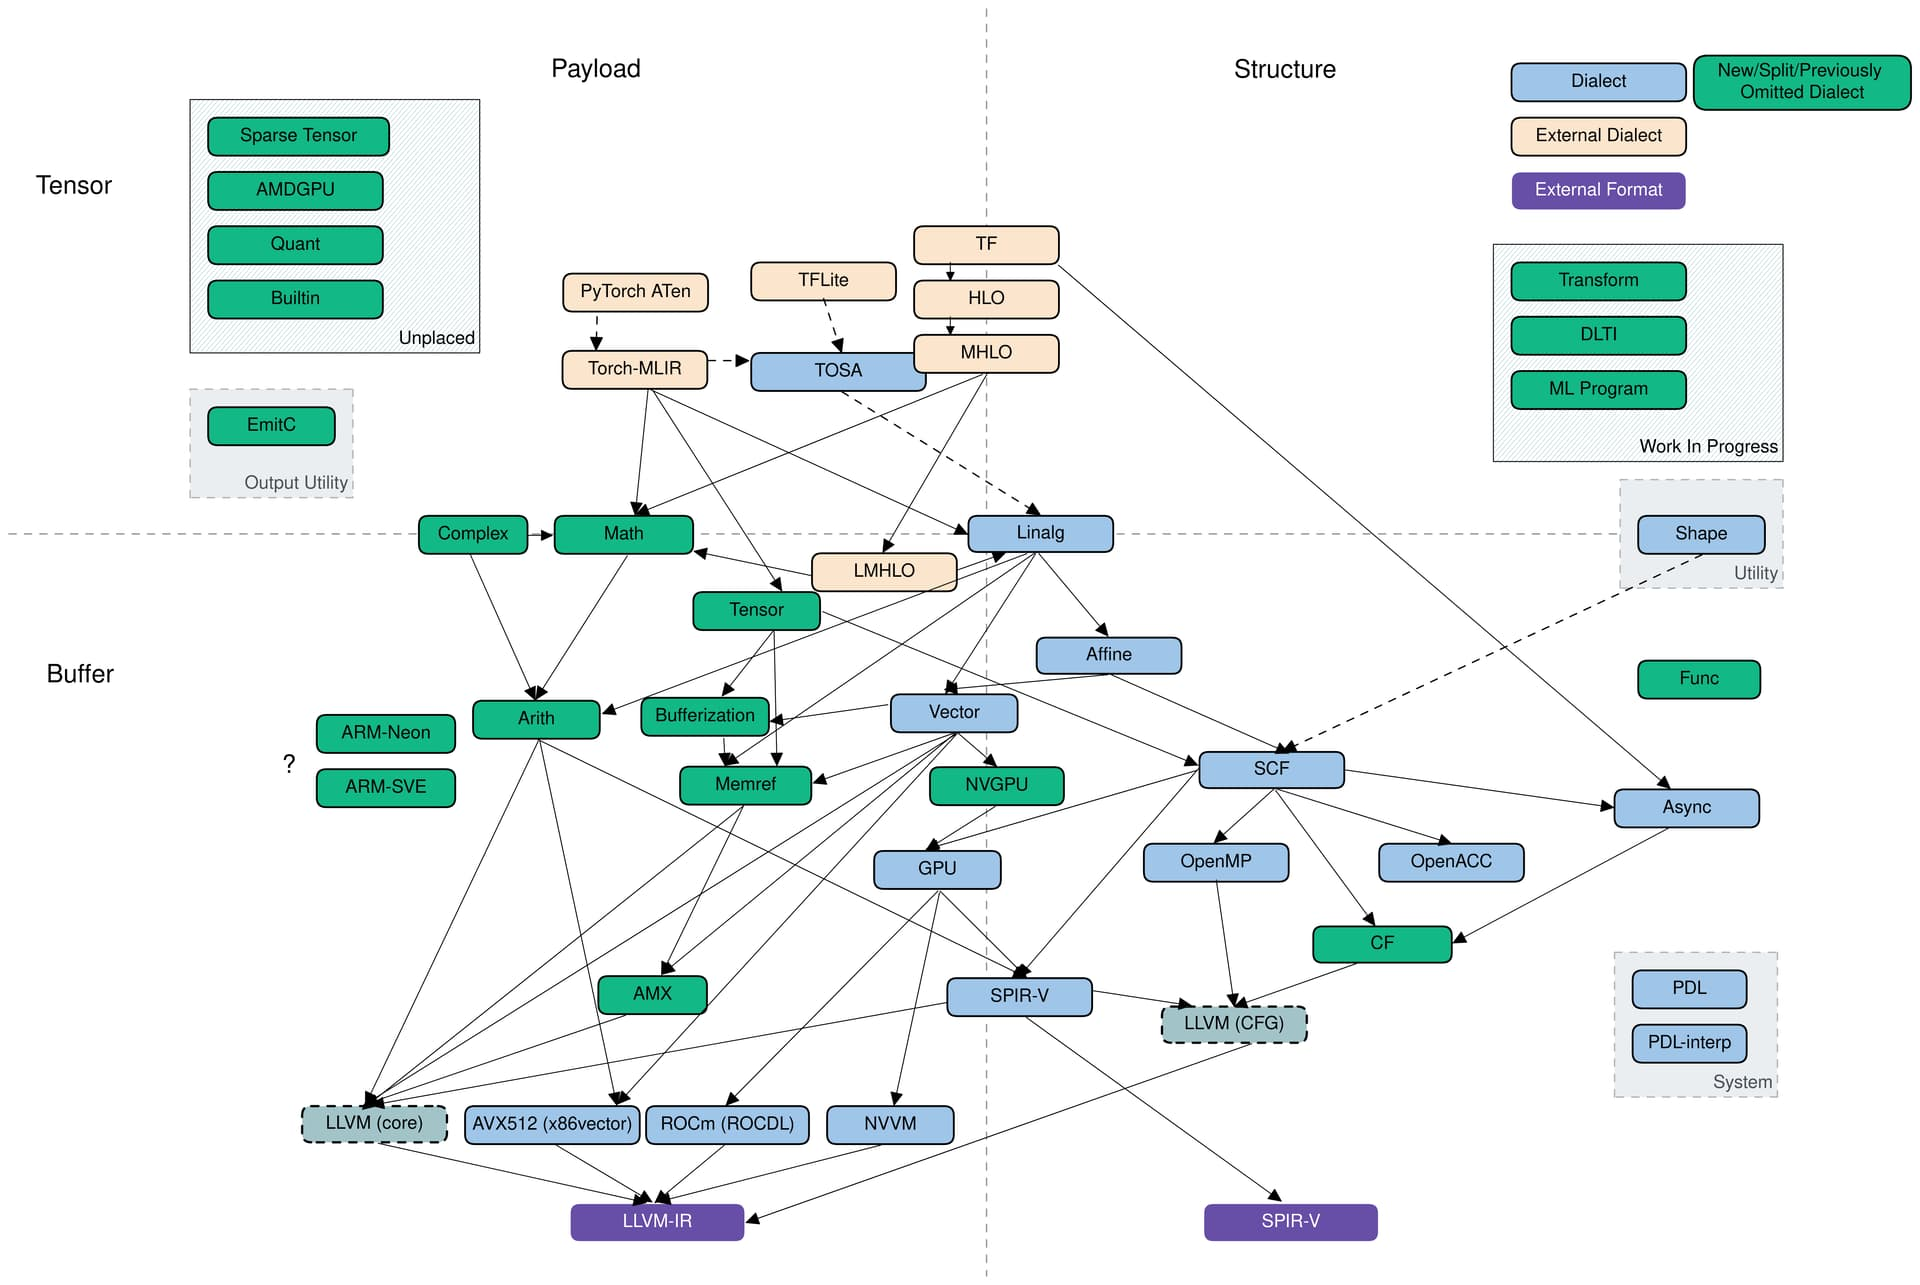
\includegraphics[scale=0.25]{MLIR_Dialects.jpg}
    \caption{Структура проекта MLIR и соотношения диалектов в них}
\end{figure}

\subsection{Функциональная структура компилятора}
\label{impl:compiler} % \index{Chapter7}

Используя знания о MLIR и DaVinci, полученные в результате исследовательской
работы, наша команда приступила к разработке нового компилятора. Было решено
создать новые диалекты, которые на разных уровнях абстракции отражают
особенности архитектуры DaVinci. Перечислим их и отметим основные особенности:

\begin{enumerate}
    \item \textit{ascend} --- диалект крупноблочных операций. Является аналогом
          HLO, но операции в нём предъявляют требования к типам данных: матрицы
          должны быть расположены в блочном формате. Поэтому в процессе ловеринга
          из HLO в ascend для входных и выходных данных вставляются операции
          фрактализации, т.е. приведения матрицы к нужному виду. Для остальных
          диалектов требование на формат данных сохраняется, при этом считается,
          что оно выполняется благодаря корректности представления графа
          исполнения в диалекте ascend.

    \item \textit{cce} --- диалект операций, схожих с ассемблерными инструкциями.
          Основная его особеннность заключается в сохранении семантики
          многомерных массивов, что позволяет упрощать процесс генерации таких
          операций и их верификации (проверки корректности).

    \item \textit{hivm} --- диалект непосредственных ассемблерных инструкций. Он в
          точности повторяет их семантику, что упрощает его ловеринг в llvm.
\end{enumerate}

Конвейер (пайплайн) компиляции для девайса выглядит следующим образом:

\begin{figure}[h!]
      \centering
      
\includegraphics[scale=0.1]{Compiler.png}
      \caption{Пайплайн компиляции для девайса}
  \end{figure}

В данной работе рассматривается ловеринг от диалекта ascend к диалекту cce,
что соответствует переходу от крупноблочных операторов к операторам, схожих с
инструкциями процессора Ascend.

\subsection{Трансляция операций и возможные стратегии}
\label{impl:lowering} % \index{Chapter8}

\newcommand{\divisible}{\mathop{\raisebox{-2pt}{\vdots}}}

Изучив особенности целевой архитектуры, перейдём к рассмотрению
конкретных стратегий трансляции и их классификации. В связи с тем, что именно
работа с внешней память занимает большую часть времени, будем пытаться
оптимизировать еë. Как было упомянуто в одной из предыдущих глав, из-за малого
объëма внутренних кэшей данные приходится загружать частями, при этом каждая часть,
возможно, будет загружена несколько раз. В связи с этим, уменьшение количества
повторных загрузок --- самый простой способ оптимизации, а стратегия разбиения,
при которой достигается наименьшее количество повторных загрузок, будет считаться
нами наиболее оптимальной.

\subsubsection{Умножение матриц}

\paragraph{Теоретическая модель}~

Умножение матриц в диалекте \texttt{ascend} представлено оператором \texttt{matmul}:

\begin{lstlisting}[caption={Пример использования оператора \texttt{matmul}}]
func.func @kernel_func(
    %matrixA: memref<48x32x16x16xf16, 1>,
    %matrixB: memref<48x48x16x16xf16, 1>,
    %matrixC: memref<48x32x16x16xf16, 1>) {
    ascend.matmul(%matrixA, %matrixB, %matrixC) : memref<48x32x16x16xf16, 1>, memref<48x48x16x16xf16, 1>, memref<48x32x16x16xf16, 1>
    return
}
\end{lstlisting}

На вход оператор примает три многомерных массива, соответствующих матрицам
$A$, $B$, $C$ матричного умножения $C = A \times B$. Все три матрицы хранятся
в формате \texttt{Nz}, это сделано для удобства, т.~к. в реальных нейронных сетях
несколько умножений могут идти подряд, при этом результат предыдущего
передаётся на вход следующего. Привести кусок матрицы к необходимому формату
(\texttt{Zz} или \texttt{Zn}) не является проблемой при правильном использовании
операций копирования из GM в L1 и загрузки из L1 в L0. Число $1$ в конце каждого
\texttt{memref} означает, что массив находится в первом адресвом пространстве, что
соответствует памяти GM.

Теперь перейдём к тому, каким образом можно реализовать трансляцию и
оптимизировать количество копирований. Согласно статье \cite{matmul-strategies}, можно выделить
три основные стратегии: \textit{input stationary (IS)}, \textit{weight stationary (WS)}
и \textit{output stationary (OS)}. Отметим, что в данной статье рассматривается
операция свёртки, но всё перечисленное в ней верно и для умножения матриц.
Все три стратегии имеют общую идею: умножение производится блочно, блок одной из
матриц <<фиксируется>> ($A$ для IS, $B$ для WS и $C$ для OS), после чего
перебираются всевозможные блоки других матриц. Наглядное объяснение этого
процесса можно увидеть на картинке. После перебора выбирается другой блок и
операция повторяется.

\begin{figure}[h!]
    \centering
    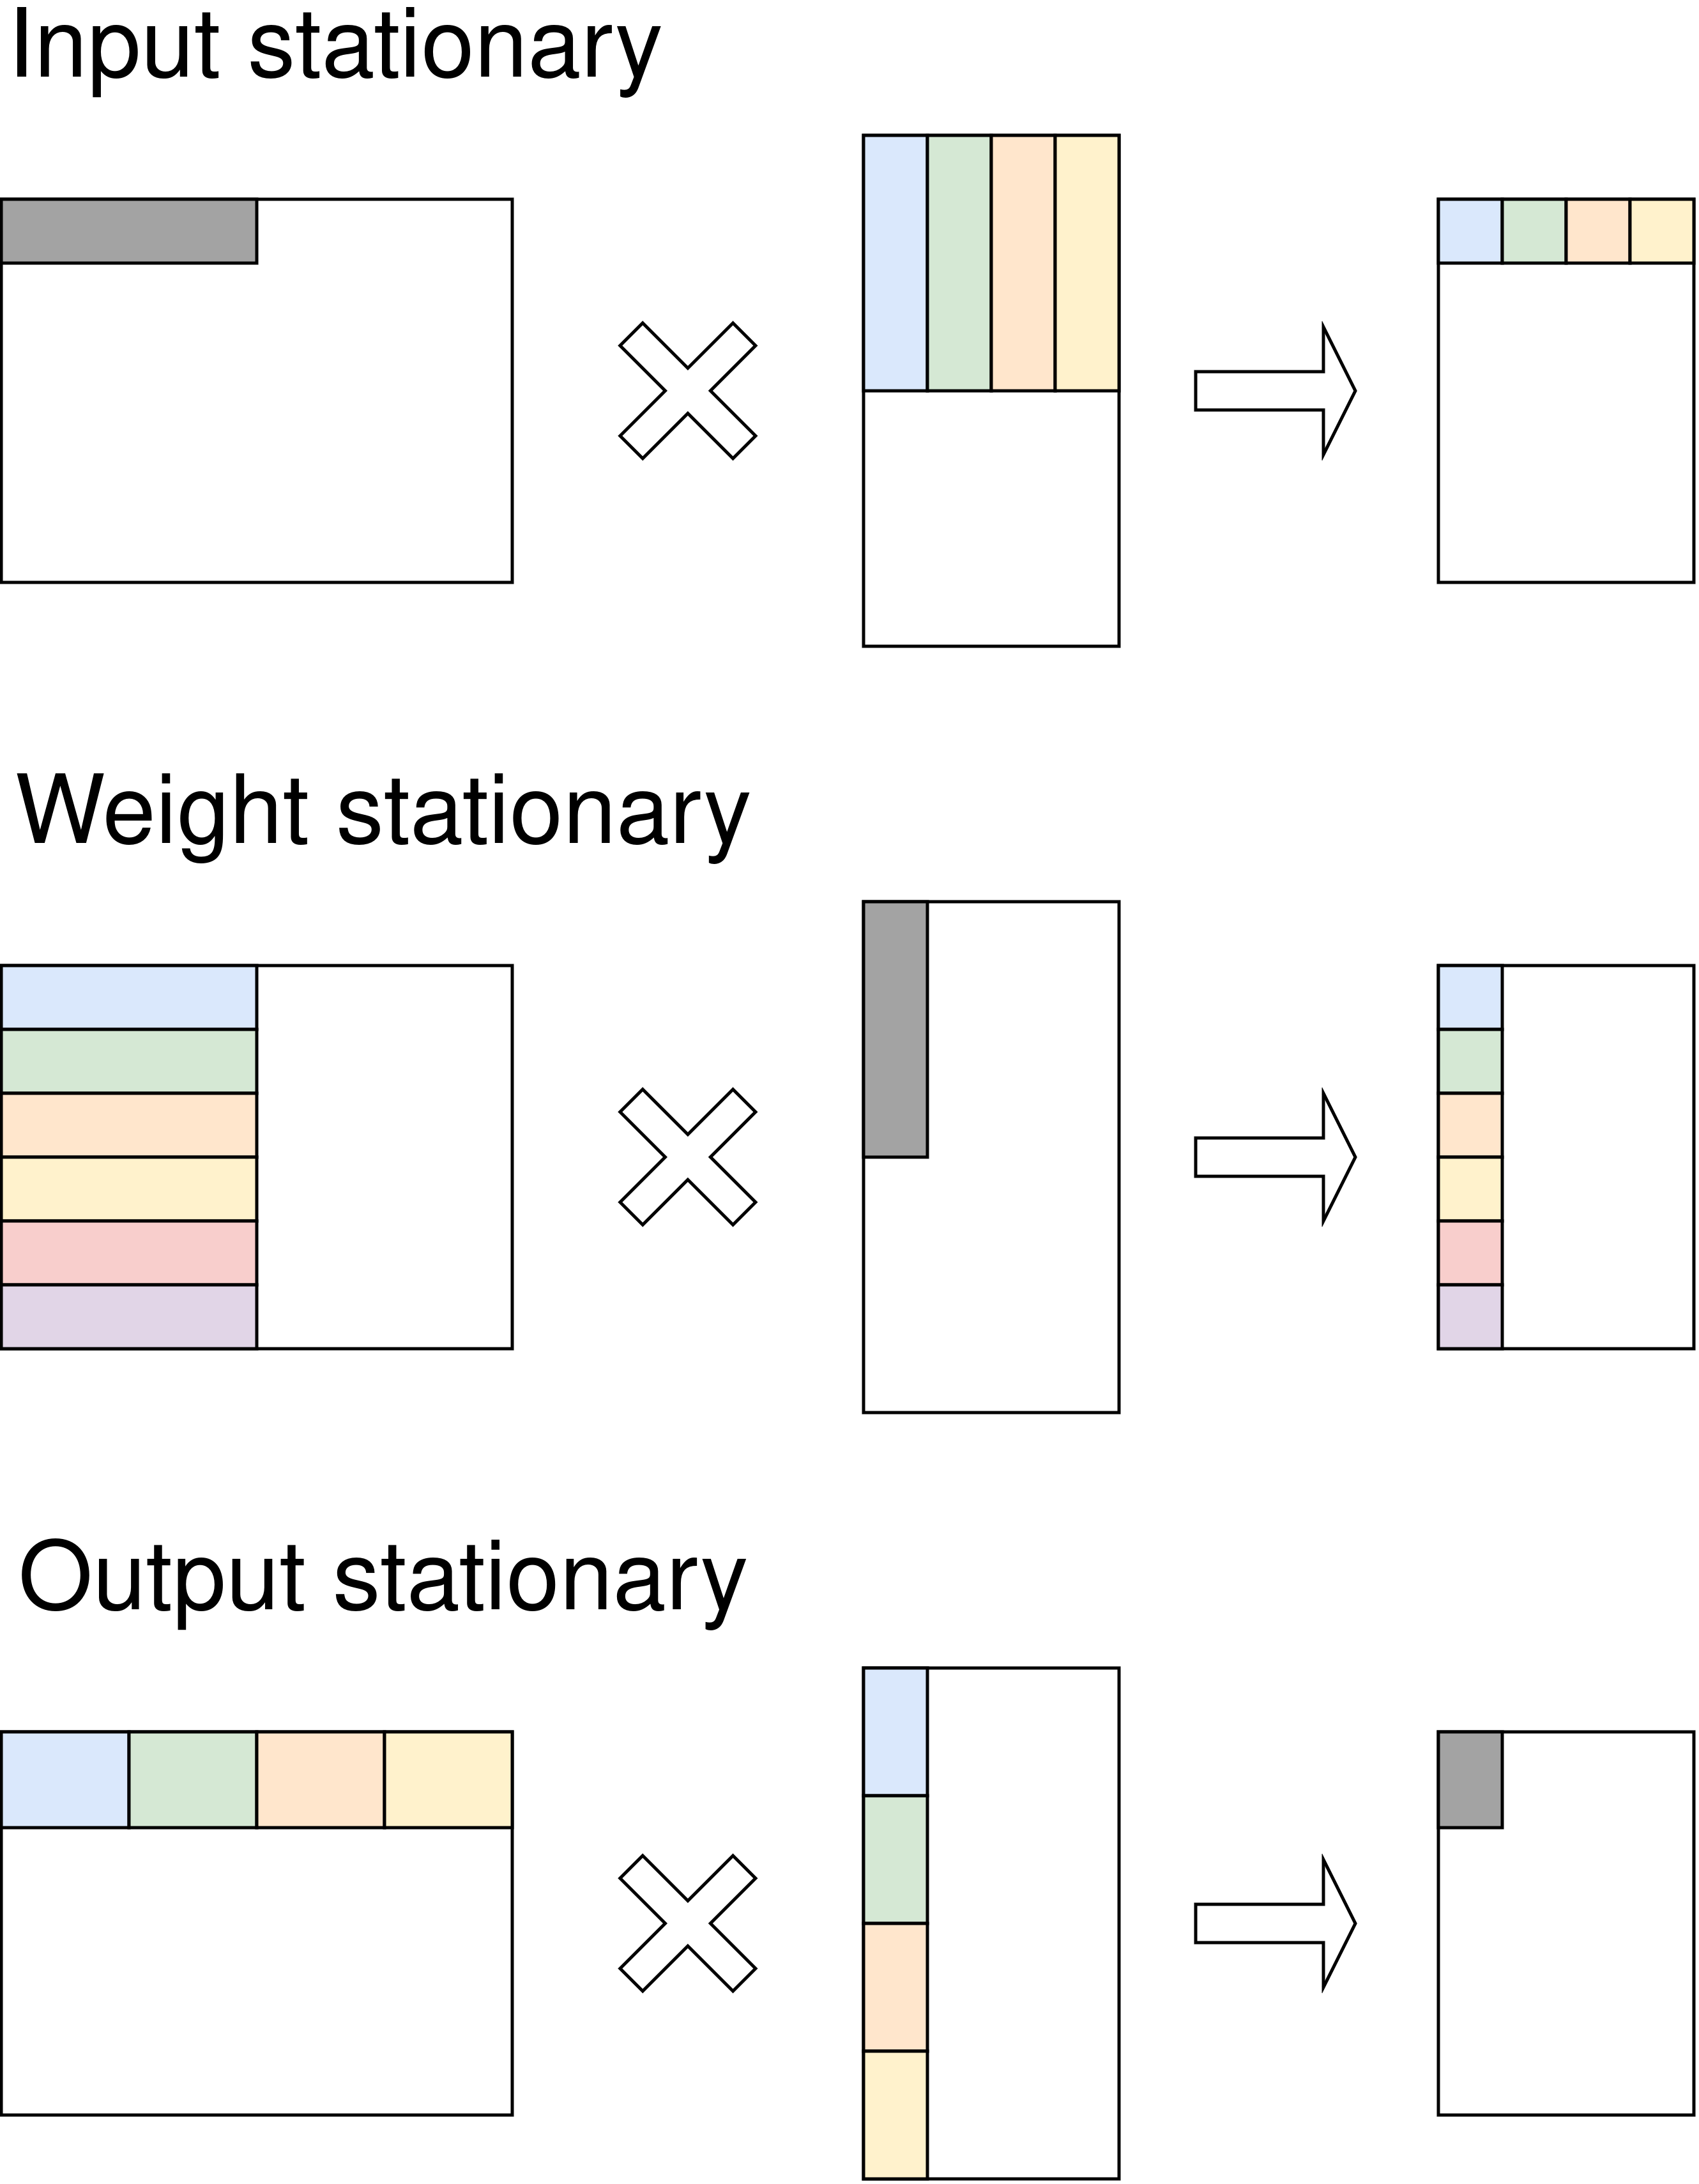
\includegraphics[scale=0.1]{Strategies.drawio.png}
    \caption{Стратегии для умножения матриц}
\end{figure}

Перечисленные стратегии описывают порядок обхода матриц по их блокам, но ничего
не говорят о размерах самих блоков. Пара стратегия + разбиение задаёт конкретное
исполнение, задача же состоит в том, чтобы выбрать исполнение, дающее
максимальную производительность. Для теоритического предсказания оптимального
исполнения нами была предложена метрика, соответствующая количеству загруженной
памяти. Опишем её более формально. Пусть матрица $A$ имеет размеры $M \times N$, а
матрица $B$ --- $N \times K$, тогда $C$ --- матрица $M \times K$. Таким образом,
матрицы описываются тройкой $(M, N, K)$. Аналогично, разбиение на блоки
описывается тройкой $(m, n, k)$. Будем рассматривать только такие конфигурации,
при которых блочное умножение можно выполнить за одну инструкцию, а выполнение
перебора блоков матриц при фиксации одного из них не требует выгрузки и загрузки
промежуточных результатов. В силу этих ограничений можно считать, что для IS
$k = K$ или $n = N$, а для WS --- $m = M$ или $n = N$.

Рассмотрим IS стратегию. Каждой загрузке матрицы $m \times n$ соответстует
$\frac{K}{k}$ загрузок матриц $n \times k$. Повторяется это действие
$\frac{MN}{mn}$ раз. Таким образом, общее количество загруженной памяти
составляет:

\[
    \Sigma_{IS} = \left( mn + nk ~ \frac{K}{k} \right) \frac{MN}{mn} = MN + \frac{MNK}{m}
\]

Аналогичным образом можно получить метрики для других стратегий:

\[
    \Sigma_{WS} = KN + \frac{MNK}{k}
\]

\[
    \Sigma_{OS} = MNK ~ \frac{m + k}{mk}
\]

На тройку $(m, n, k)$ должны быть наложены ограничения, связанные с размерами буферов.
Если считать, что элементы входных матриц имеют тип \texttt{float 16}, а выходной ---
\texttt{float 32} (это соответствует вычислениям на Ascend с повышенной точностью) тогда:

\[
\begin{cases}
    M, N, K, m, n, k \divisible 16 \\
    mn \leqslant 2^{15} \\
    nk \leqslant 2^{15} \\
    mk \leqslant 2^{16}
\end{cases}
\]

Итак, загружаемая память должна быть минимизирована, т.~е. $\Sigma \rightarrow \min$
Из эмпирических наблюдений (речь о которых пойдёт далее), при прочих равных используемая
память должна быть максимизирована:

\[
\begin{cases}
    mn \rightarrow \max \\
    nk \rightarrow \max \\
    mk \rightarrow \max
\end{cases}
\]

\paragraph{Экспериментальная модель}~

Для проверки гипотезы был разработан тестовый бенчмарк, замеряющий время
исполнения при различных конфигурацях и оптимизациях (см. главу
\ref{subsubsec:Opt}). Напомним, что исполнение задаётся стратегией и двумя
тройками $(M, N, K)$ и $(m, n, k)$, обозначающими размеры целой матрицы и блоков
разбиения. Рассмотрим пример, типичный для нейросети BERT:
$(M, N, K) = (512, 768, 768)$. Путём перебора был найден минимум метрики
$\Sigma = 2359296$ в случае OS стратегии при $m = k$.  Рассмотрим различные
$m$ и $k$, проварьируем $n$ и рассмотрим возможные (подходящие под ограничения)
OS-исполнения. Соответствующие графики представлены ниже.

\begin{figure}[h!]
    \centering
    \begin{subfigure}{0.45 \textwidth}
        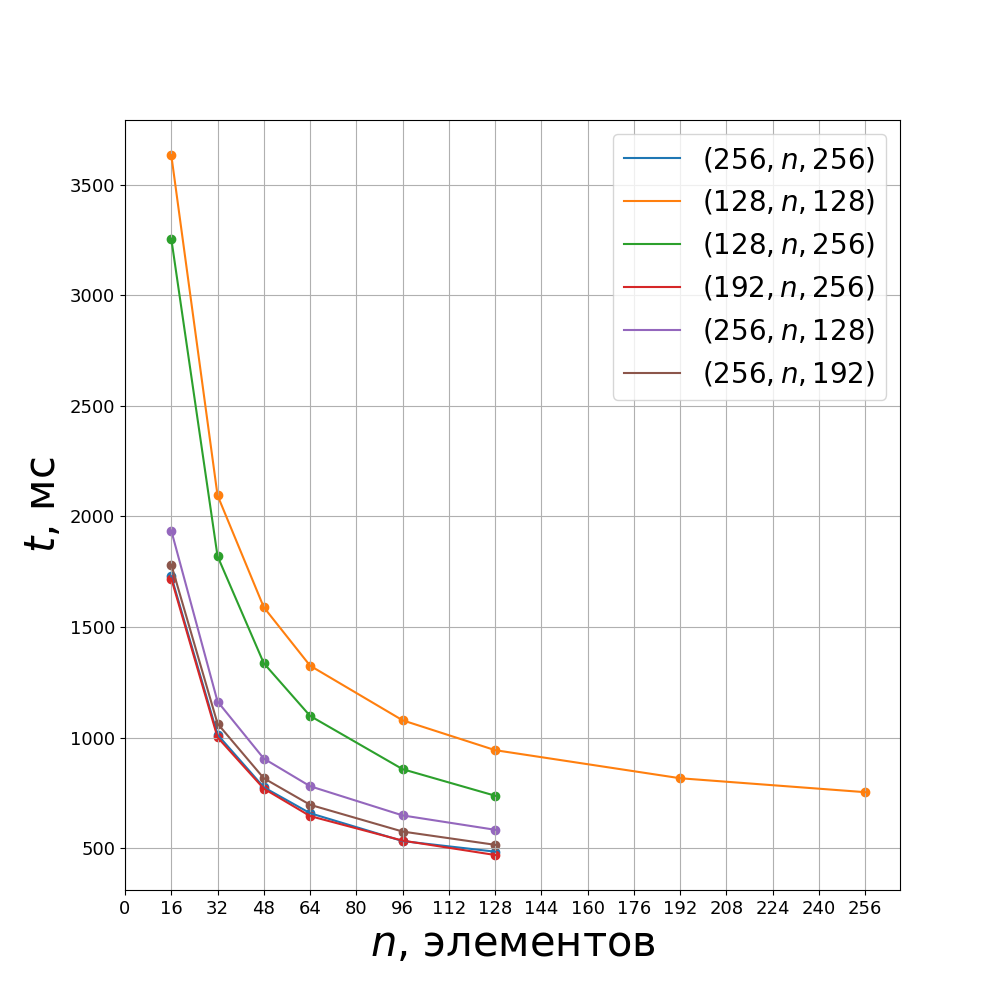
\includegraphics[scale=0.3]{simple.png}
        \caption{Без оптимизаций}
    \end{subfigure}
    ~
    \begin{subfigure}{0.45 \textwidth}
        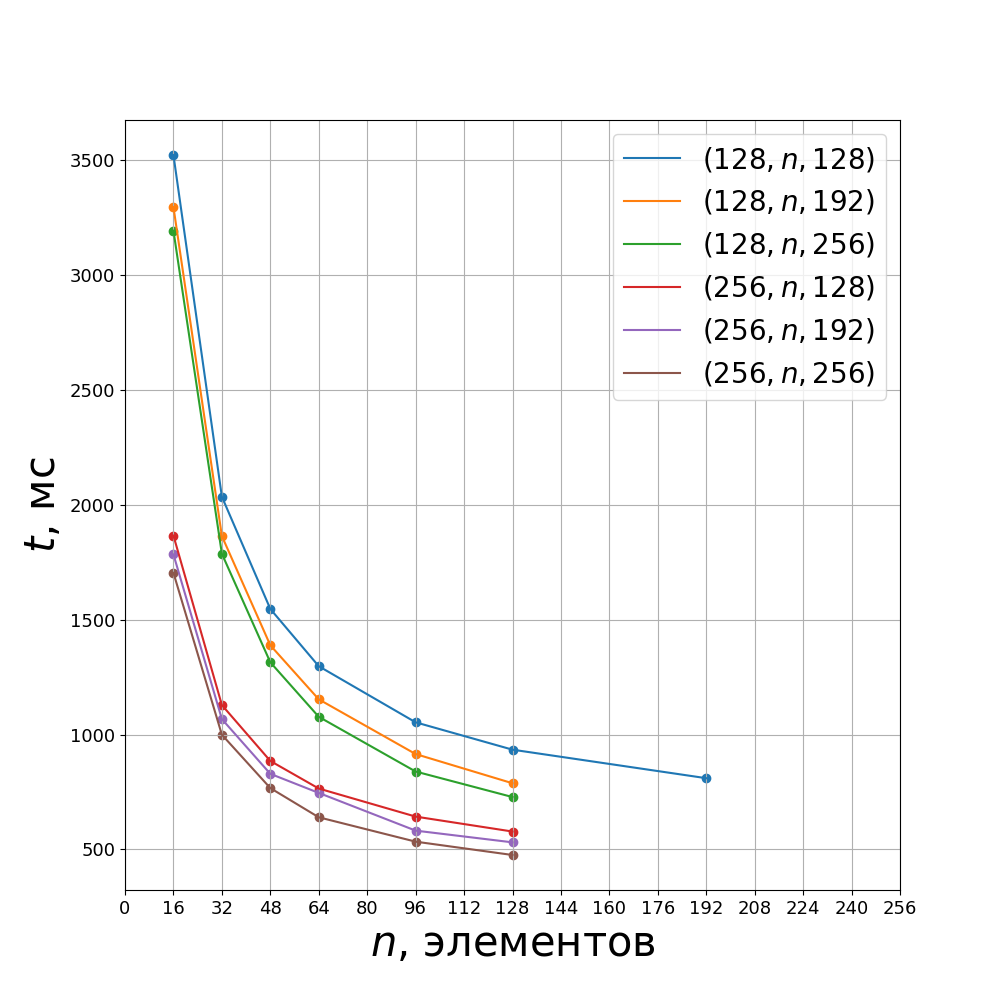
\includegraphics[scale=0.3]{db.png}
        \caption{С двойной буферизацией}
    \end{subfigure}
\end{figure}
\begin{figure}[h!]
    \begin{subfigure}{0.45 \textwidth}
        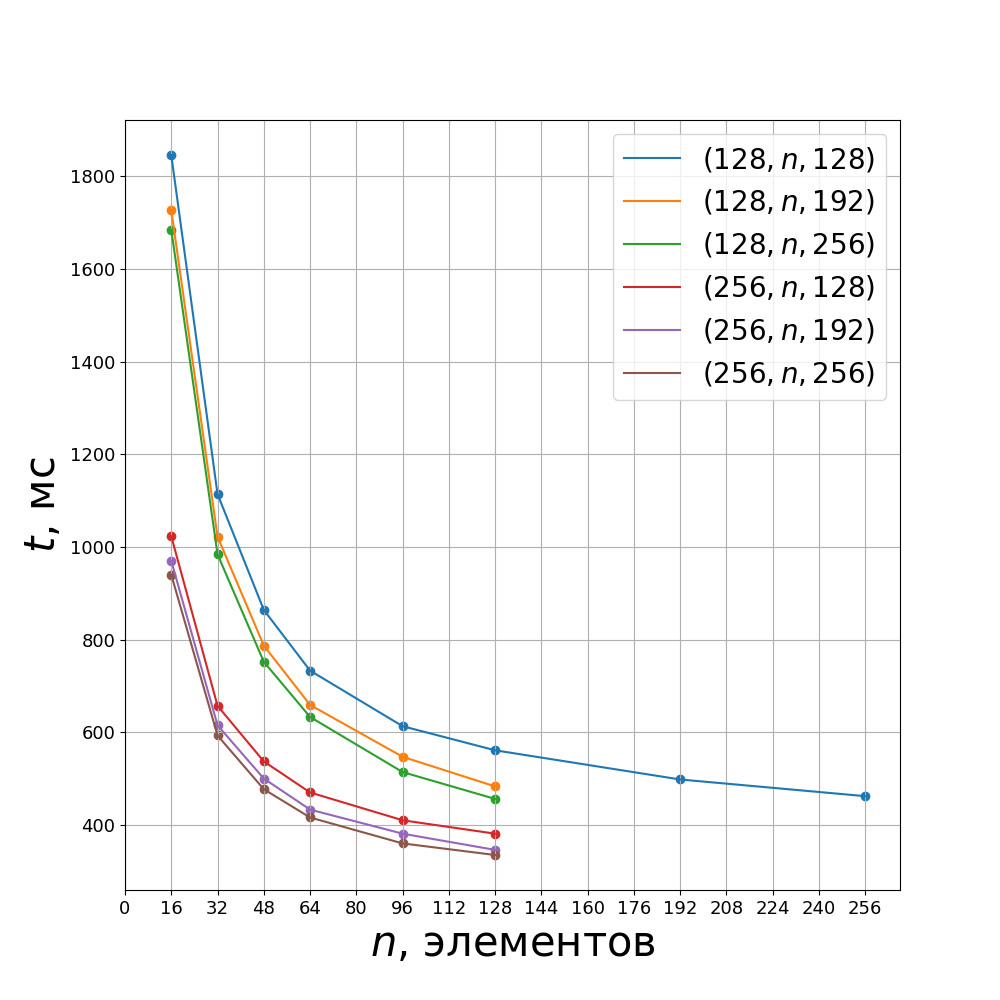
\includegraphics[scale=0.3]{2t.png}
        \caption{С распараллеливанием}
    \end{subfigure}
    ~
    \begin{subfigure}{0.45 \textwidth}
        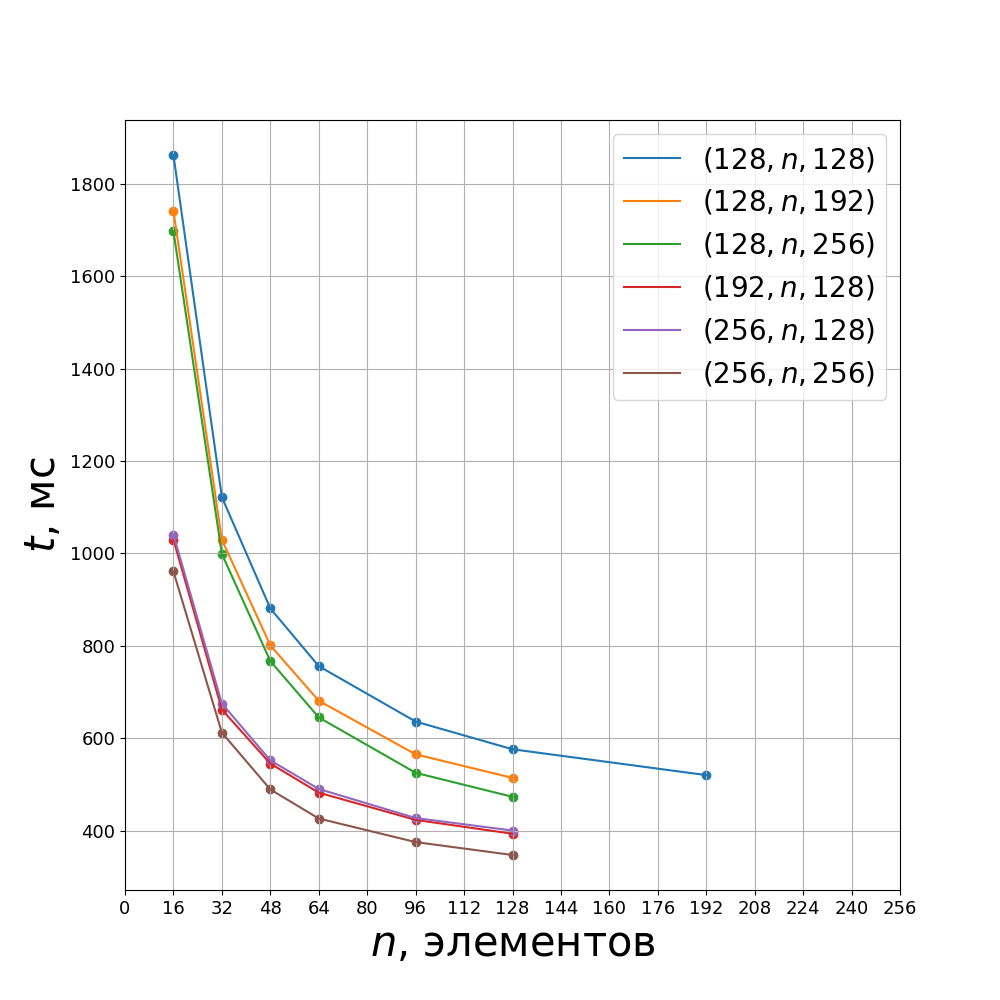
\includegraphics[scale=0.3]{db_2t.png}
        \caption{С двойной буферизацией и распараллеливанием}
    \end{subfigure}
\caption{Зависимость времени работы от параметра разбиения $n$}
\end{figure}

Также сравним наиболее оптимальные исполнения IS --- $(32, 768, 32)$,
WS --- $(32, 768, 32)$ и OS --- $(256, 128, 256)$. Диаграмма
для случая без оптимизаций представлена ниже.

\begin{figure}[h!]
    \centering
    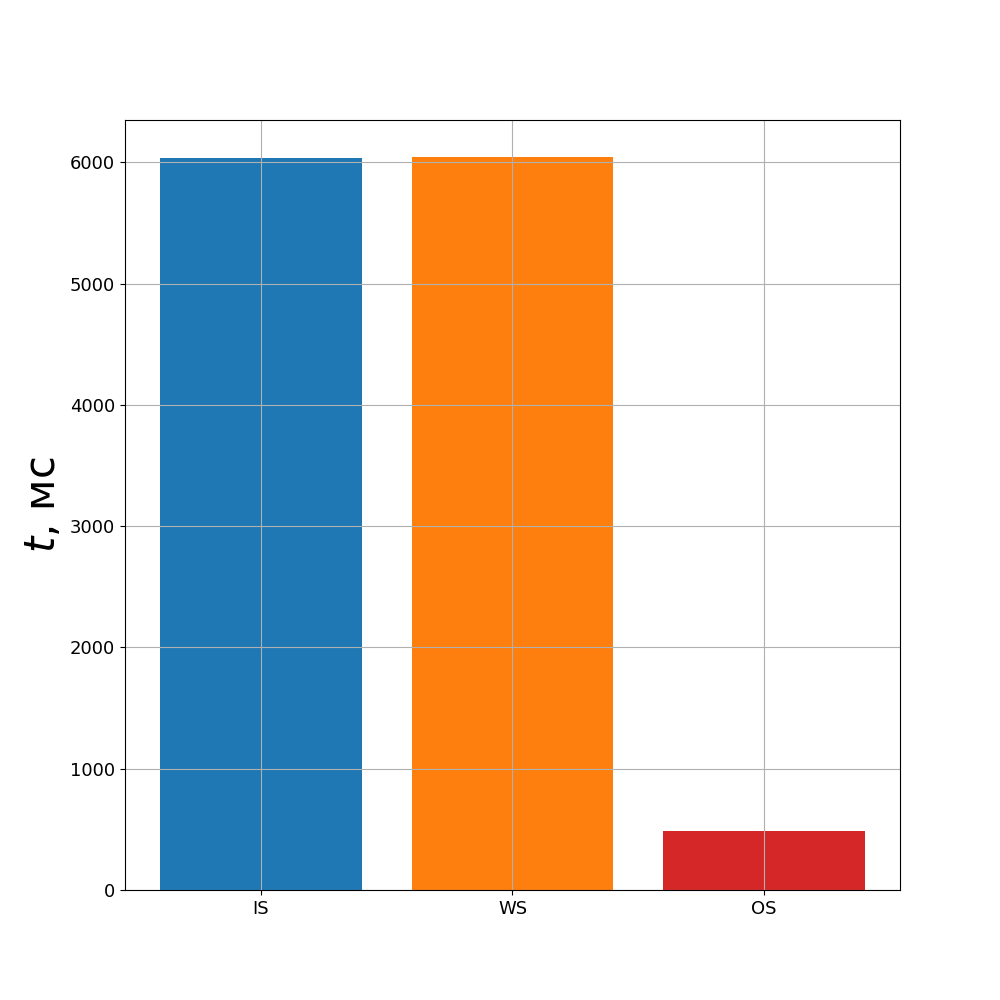
\includegraphics[scale=0.33]{time_diagram.png}
    \caption{Сравнение производительности различных стратегий}
\end{figure}

Гипотеза, изложенная выше, частично подтвердилась.
Если рассматривать типичные размеры умножаемых матриц в нейросетях (например,
BERT) --- $(512, 768, 768)$, то оказывается, что OS --- наиболее оптимальная
стратегия, а $(256, 128, 256)$ --- оптимальная конфигурация. Конфигурация
$(128, 256, 128)$ не является оптимальной, несмотря на текущую теоритическую
модель, т.~к. в ней не учитываются выгрузки памяти.

\paragraph{Реализация}~

OS стратегия была реализована в компиляторе на инфраструктуре MLIR в виде
понижения оператора \texttt{ascend.matmul} до цикла на диалектах cce,
affine и memref. Ниже приведён псевдокод алгоритма:

\begin{lstlisting}[caption={Алгоритм умножения матриц}]
func ascend.matmul(matrixA, matrixB, matrixC) {
    for (x = [0, M / m)) {
        for (y = [0, K / k)) {
            c = empty_buf(m, k)
            for (sum_part = [0, N / n)) {
                a = empty_buf(m, n)
                b = empty_buf(n, k)
                load_part(a, matrixA, sum_part, y)
                load_part(b, matrixB, x, sum_part)
                cce.mad(a, b, c)
            }
            store_part(matrixC, c, x, y)
        }
    }
}
\end{lstlisting}

Подчеркнём, что в реальности алгоритм имеет несколько особенностей, не
отражённых в псевдокоде. Во-первых, учитывается фрактализация матриц (их формат
хранения). Несмотря на то, что в L0A и L0B матрицы должны лежать в формате Zz и Zn
соответственно, в памяти GM они хранятся в формате Nz (это сделано для выполнения
нескольких умножений подряд без выполнения промежуточных фрактализаций). Изменение
формата происходит в ходе загрузки матриц во внутренни буферы. Во-вторых,
операции, названные в псевдокоде \texttt{load\_part} для $A$ и $B$ и \texttt{store\_part}
для $C$, состоят из двух этапов, для каждой матрицы по-разному:
$A: GM \rightarrow L1 \rightarrow L0A$, $B: GM \rightarrow L1 \rightarrow L0B$,
$C: L0C \rightarrow UB \rightarrow GM$. В-третьих, поддержана операция
\texttt{ascend.batch\_matmul}, которая производит умножение нескольких пар матриц.

\subsubsection{Фрактализация и дефрактализация}

Как было написано ранее, перемножение матриц требует особый формат хранения,
при этом было решено передавать на вход оператора умножения в формате Nz.
По этой причине необходимо матрицы, поступающие на вход нейронной сети, заранее
фрактализовать (т.е. поменять формат хранения). Обратное действие
(дефрактализация) необходимо для матрицы на выходе. Отметим, что далее речь
будет идти только о фрактализации, т.к. все преобразования линейны и
дефрактализация будет представлять собой действия фрактализации, выполненные в
обратном порядке. Рассмотрим фрактализацию на примере матрицы
$(512 \times 768)$. В формате Nz она будет иметь вид
$48 \times 32 \times 16 \times 16$. В скалярном коде фрактализация имеет
следующий вид:

\begin{lstlisting}[caption={Скалярный код фрактализации}]
half src[512][768];
half dst[48][32][16][16];

for (i = [0, 48))
  for (j = [0, 32))
    for (k = [0, 16))
      for (l = [0, 16))
        dst[i][j][k][l] = src[j * 16 + k][i * 16 + l];
\end{lstlisting}

Исполнение скалярного кода является медленным, по этой причине будем
использовать инструкцию scatter\_vnchwconv. Было реализовано два алгоритма.

\textit{Наивный алгоритм} работает циклом с частями $16 \times 768$, первый
scatter собирает матрицы в блоки $16 \times 16$, а второй транспонирует
блоки. Для преобразования всей матрицы происходит перебор этих кусочков,
а копирование в GM происходит по блокам с шагом 32 блока.

\begin{lstlisting}[caption={Наивный алгоритм фрактализации}]
half src[16][768];
half tmp[48][16][16]
half dst[48][16][16];

scatter_vnchwconv(
    src = src, dst = tmp,
    src_ptrs = {{0, 0}, {1, 0}, {2, 0}, ...},
    dst_ptrs = {{0, 0, 0}, {0, 1, 0}, {0, 2, 0}, ...},
    src_stride = {0, 16},
    dst_stride = {1, 0, 0},
    repeat = 48
);

scatter_vnchwconv(
    src = tmp, dst = dst,
    src_ptrs = {{0, 0, 0}, {0, 1, 0}, {0, 2, 0}, ...},
    dst_ptrs = {{0, 0, 0}, {0, 1, 0}, {0, 2, 0}, ...},
    src_stride = {1, 0, 0},
    dst_stride = {1, 0, 0},
    repeat = 48
);
\end{lstlisting}

\textit{Улучшенный алгоритм} позволяет задействовать всю память UB:

\begin{lstlisting}[caption={Продвинутый алгоритм фрактализации}]
half src[80][768];
half tmp[5][48][16][16]
half dst[48][16][5][16];

half src_reshape[16][5][48][16] = reshape(src)

scatter_vnchwconv(
    src = src_reshape, dst = tmp,
    src_ptrs = {{0, 0, 0, 0}, {1, 0, 0, 0}, {2, 0, 0, 0}, ...},
    dst_ptrs = {{0, 0, 0, 0}, {0, 0, 1, 0}, {0, 0, 2, 0}, ...},
    src_stride = {0, 0, 1, 0},
    dst_stride = {0, 1, 0, 0},
    repeat = 240
);

for (i = [0, 5))
    scatter_vnchwconv(
        src = tmp, dst = src,
        src_ptrs = {{i, 0, 0, 0}, {i, 0, 1, 0}, {i, 0, 2, 0}, ...},
        dst_ptrs = {{0, 0, i, 0}, {0, 1, i, 0}, {0, 2, i, 0}, ...},
        src_stride = {0, 1, 0, 0},
        dst_stride = {1, 0, 0, 0},
        repeat = 48
    );

half dst_logical_shape[48][5][16][16] = reshape(dst)
\end{lstlisting}

С его помощью обрабатывается часть $80 \times 768$. После разбиения матрицы
на части остаётся <<хвост>> $32 \times 768$, который обрабатывается аналогично.
Загрузка результата в GM происходит по 5 блоков. Отметим, что операция reshape
является исключительно логической и не изменяет порядок хранения элементов.

\subsubsection{Поэлементные операции}

На момент написания текста были реализованы некоторые бинарные операции
(сложение, вычитание, умножение, деление, максимум, минимум), преобразование
типов и операция <<зажима>>: $clamp(x, y, z) = \min(z, \max(x, y))$. Все они
работают по общему приниципу: если массив данных многомерный, он преобразуется
к одномерному. Далее массив разбивается на максимально возможные порции,
при которых в UB помещаются входные и выходные данные. Данные загружаются из
GM порциями, обрабатываются соответствующими векторными операциями и ответ
выгружается. Отметим, что в силу того, что количество элементов в порции
может быть некратным количеству элементов, обрабатываемых за итерацию инструкции
(128 в случае \texttt{float 16} и 64 в случае \texttt{float 32} или
\texttt{int 32}), конец порции необходимо обработать отдельно, предварительно
изменив маску.

Также может возникнуть проблема, связанная с обработкой последней порции и
гранулярностью UB. Напомним, что в UB возможна заргузка данных, размер которых
кратен 32 байтам. Это означает, что если размер всего массива данных не кратен
32, то с загрузкой последней порции могут возникнуть случае. Решением этой
проблемы является загрузка <<с наложением>>: загрузка некоторую часть предыдущей
порции с целью выровнять размер. При этом это <<наложение>> обрабатывается и
выгружается повторно. Отметим, что такая схема не влияет на общую
производительность, т.~к. размер <<наложения>> пренебрежимо мал по сравнению
с размерами всего массива.

Пример псевдокода для операции cast представлен ниже:

\begin{lstlisting}[caption={Алгоритм оператора \texttt{cast}}]
half src[N];
float dst[N];

size_t n = pick_max_available(N);
half src_local[n];
float dst_local[n];

for (i = [0, N / n))
    copy(src + i * n, src_local, n);
    cast_f16_f32(
        src = src_local, dst = dst_local,
        repeat = n / 64, mask = full_mask,
        src_stride = 4 blocks, // 64 elems
        dst_stride = 8 blocks // 64 elems
    );
    copy(dst_local, dst + i * n, n);

// tail handling with overlapping
size_t block_size = 16;
size_t tail = (N % n + block_size - 1) / block_size * block_size;

copy(src + N - tail, src_local, tail);
cast_f16_f32(
    src = src_local, dst = dst_local,
    repeat = 1, mask = partial_mask,
    src_stride = 0 blocks, // only one repeat
    dst_stride = 0 blocks // only one repeat
);
copy(dst_local, dst + N - tail, tail);
\end{lstlisting}

\subsubsection{Транспонирование}

Операция транспонирования в моделях нейронных сетей работает с многомерными
тензорами, по этой причине данную операцию корректнее называть <<перестановкой
измерений>>. В каком-то смысле эта операция является изменением формата хранения
данных, но более общим случаем. На данный момент поддержаны операции из BERT,
их можно представить в двух формах:

\textit{Первая форма} выражается формулой $dst_{ijk} = src_{ikj}$, т.~е.
является транспонированием нескольких матриц. Решается задача аналогично
поэлементным операциям за тем лишь исключением, что в данном случае используется
инструкция \texttt{scatter\_vnchwconv}, которая работает с матрицами
$16 \times 16$, что является гранулярностью в данном случае. Проблема, связанные
с гранулярностью, решается аналогично: алгоритм использует схему <<с наложением>>.

\textit{Вторая форма} выражается формулой $dst_{ijkl} = src_{ikjl}$. В данном
случае алгоритм осуществляет поблочное копирование из преположения, что размер
младшего измерения кратен 32 байтам.

\subsubsection{Трансляция диалектов cce и hivm}

Рассмотрим трансляцию из диалекта cce в hivm.
Напомним (см. главу \ref{impl:compiler}), что диалект cce соответствует целевым
инструкциям, но сохраняет семантику многомерных массивов, а в hivm эта семантика
отсутствует. По этой причине многомерные массивы (\texttt{memref}) преобразуются
в указатели (\texttt{llvm.ptr}), при необходимости использования части буфера,
не совпадающей с началом, используется адресная арифметика, представленная
оператором \texttt{llvm.getelementptr}. Все размеры в операции копирования
пересчитываются на размеры блоков (например, копирование
\texttt{memref<1x16x1xf16>} соответствует копированию 32 байт, т.~е. одному блоку
UB).

При трансляции из hivm в llvm происходит \textit{упаковка параметров}.
Ассемблерные инструкции процессора Ascend принимают аргументы в виде
\textit{конфигурационного числа} размером 64 бита. Разные биты обозначают
различные аргументы инструкции. Например, во многих инструкциях биты с 56 по 63
соответствуют количеству повторений внутри инструкции (см. \ref{subsubsec:vec}).
По этой причине при трансляции hivm все аргументы инструкции размещаются на своих
позициях с помощью побитовой арифметики, позиции были получены путём реверс
инжиниринга. Отметим, что аргументы могут быть динамическими, по этой причине
конфигурационное число вычисляется во время исполнения.


\newpage

    \section{Заключение и дальнейшая работа}
\label{sec:Conclusion} \index{Conclusion}

В рамках данной работы были решены следующие задачи:

\begin{enumerate}
    \item Исследованы архитектуры нейронных сетей BERT и ResNet,
          основными целями для реализации были выбраны умножение матриц и
          векторные операции.
    \item Исследованы различные инфраструктуры для создания и компиляции
          нейронных сетей (например, PyTorch, Tensorflow), и используемые ими
          аппаратные возможности для увеличения производительности.
    \item Разработан набор операторов для целевой архитектуры DaVinci в
          инфраструктуре MLIR (диалекты CCE и HIVM).
    \item Разработан набор тестов для оценки эффективности стратегий трансляции
          операций нейронных сетей.
    \item Реализованы методы генерации целевых инструкций процессора
          для операций умножения матриц, фрактализации, векторных операций.
\end{enumerate}


Корректность трансляции каждой крупноблочной операции из главы
\ref{impl:lowering} была проверена на синтетическом наборе тестов. Результат
работы оператора сравнивался с эталонным результатом, полученным при исполнении
аналогичного кода на языке Python. Корректность работы всего компилятора
экспериментально исследована и подтверждена на реальной нейронной сети BERT,
содержащей 478 операторов.

Но, несмотря на это, планируются дальнейшие исследования.
На данный момент компилятор находится в стадии активной разработки, поэтому
отметим проблемы, которые были выяснены в процессе исследования и будут решены
в будущем:

\begin{enumerate}
    \item Процессоры Ascend содержат несколько ядер, по этой причине разделение
          крупноблочных операций на несколько независимых частей является одним
          из наиболее простых способов увеличить производительность (см.
          главу \ref{subsubsec:Opt}).
    \item Замеры производительности показали, что двойная буферизация (см.
          главу \ref{subsubsec:Opt}) повышают производительность.
    \item Инструменты синхронизации в текущем компиляторе используются
          неоптимально, улучшение алгоритмов синхронизации ведёт к снижению
          времени исполнения.
    \item Методы полиэдральной компиляции (см. главу \ref{subsec:poly})
          могут быть использованы для оптимизации гнёзд циклов. Необходимы
          дополнительные исследования для изучения этих возможностей.
    \item В операциях нейронных сетей многомерные массивы могут иметь динамические
          размеры (т.~е. неизвестные на этапе компиляции), на данный момент
          их поддержка отсутствует.
\end{enumerate}

\newpage


    %% НЕ ТРОГАЙТЕ!!!
    \nocite{*}
    \bibliography{references}

    %% в зависимости от надобности подключаем раздел "Приложение"
    % \newpage
    % \input{Appendix.tex}
\end{document}
